% Define document class
\documentclass[twocolumn]{aastex631}
\usepackage{showyourwork}

\usepackage[acronym]{glossaries}
\usepackage{rotating}

% Commands
\newcommand{\gweventid}{S230922g}
\newcommand{\gwemopt}{\texttt{gwemopt}}
\newcommand{\postgresql}{\texttt{PostgreSQL}}
\newcommand{\todo}[1]{\textbf{\color{red} #1}}
\newcommand{\Nfollowuppointings}{\todo{Nfollowuppointings}}
\newcommand{\followupprobabilitycoverage}{\todo{followupprobabiltycoverage}}
\newcommand{\followupstarttime}{\todo{HH:MM UT}}
\newcommand{\detectionexptime}{\todo{HH:MM UT}}
\newcommand{\teff}{t_{\rm eff}}

% Acronyms
\newacronym{gw}{GW}{gravitational wave}
\newacronym{grb}{GRB}{gamma ray burst}
\newacronym{ns}{NS}{neutron star}
\newacronym{bh}{BH}{black hole}
\newacronym{bns}{BNS}{binary \gls{ns}}
\newacronym{bbh}{BBH}{binary \gls{bh}}
\newacronym{em}{EM}{electromagnetic}
\newacronym[plural=AGNs, firstplural=active galactic nuclei]{agn}{AGN}{active galactic nucleus}
\newacronym{sfft}{\texttt{SFFT}}{\texttt{Saccadic Fast Fourier Transform}}
\newacronym{lvk}{LVK}{LIGO/Virgo/KAGRA}
\newacronym{o4}{O4}{the fourth \gls{lvk} observing run}
\newacronym{psc}{PSC}{Pittsburgh Supercomputing Center}
\newacronym{nersc}{NERSC}{National Energy Research Scientific Computing Center}
\newacronym{decam}{DECam}{Dark Energy Camera}
\newacronym{cp}{CP}{Community Pipeline}
\newacronym{des}{DES}{Dark Energy Survey}
\newacronym{desi}{DESI}{Dark Energy Spectroscopic Instrument}
\newacronym{decals}{DECaLS}{\gls{decam} Legacy Survey}
\newacronym{delve}{DELVE}{\gls{decam} Local Volume Exploration survey}
\newacronym{ls}{LS}{\gls{desi} Legacy Survey}
\newacronym{mpc}{MPC}{Minor Planet Center}
\newacronym{tns}{TNS}{Transient Name Server}
\newacronym{cbc}{CBC}{compact binary coalescence}
\newacronym{gcn}{GCN}{General Coordinates Network}
\newacronym[plural=KNe, firstplural=kilonovae]{kn}{KN}{kilonova}
\newacronym{too}{ToO}{Target of Opportunity}
\newacronym{healpix}{HEALPix}{Hierarchical Equal Area isoLatitude Pixelation}
\newacronym{gwmmads}{GW-MMADS}{Gravitational Wave Multi-Messenger Astronomy DECam Survey}
\newacronym{snr}{SNR}{signal-to-noise ratio}
\newacronym{noirlab}{NOIRLab}{National Optical-Infrared Astronomy Research Laboratory}
\newacronym{cnn}{CNN}{Convolutional Neural Network}
\newacronym{parsnip}{ParSNIP}{Parameterization of SuperNova Intrinsic Properties}
\newacronym[plural=SNe, firstplural=supernovae]{sn}{SN}{supernova}

% - pipeline description
% - selection criteria
% - photometry of candidates
% - spectroscopic follow-up
%    - fix Gemini spectrum
% - plot of most interesting events on Light in the Dark parameter plot (figure 2)
%     - write code to fit LitD model to our lightcurves
% - Ariel's fitting/BPT diagram
%     - confirm that the uncertainties are ~4x the value

% Begin!
\begin{document}

% Title
\title{First gravitational wave follow-up of the Fourth LIGO/Virgo/KAGRA Observing Run with DECam: the case of S230922g}

\shorttitle{S230922g GW-MMADS Follow-up}

% Author list
\author[0000-0002-1270-7666]{Tom\'as Cabrera}
\affiliation{McWilliams Center for Cosmology,
    Department of Physics,
    Carnegie Mellon University,
    5000 Forbes Avenue, Pittsburgh, PA 15213
}

\author[0000-0002-6011-0530]{Antonella Palmese}
\affiliation{McWilliams Center for Cosmology,
    Department of Physics,
    Carnegie Mellon University,
    5000 Forbes Avenue, Pittsburgh, PA 15213
}

\author{Igor Andreoni}
\affiliation{}

\author{Lei Hu}
\affiliation{McWilliams Center for Cosmology,
    Department of Physics,
    Carnegie Mellon University,
    5000 Forbes Avenue, Pittsburgh, PA 15213
}

\author{Brendan O'Connor}
\affiliation{McWilliams Center for Cosmology,
    Department of Physics,
    Carnegie Mellon University,
    5000 Forbes Avenue, Pittsburgh, PA 15213
}

\author{Ariel Amsellem}
\affiliation{McWilliams Center for Cosmology,
    Department of Physics,
    Carnegie Mellon University,
    5000 Forbes Avenue, Pittsburgh, PA 15213
}

\author{Veronica Diaz}
\affiliation{McWilliams Center for Cosmology,
    Department of Physics,
    Carnegie Mellon University,
    5000 Forbes Avenue, Pittsburgh, PA 15213
}

\author{Saavik Ford}
\affiliation{}

\author{Matthew Graham}
\affiliation{}

\author{Daniel Gruen}
\affiliation{}

\author{Barry McKernan}
\affiliation{}

\author{Keerthi Kunnumkai}
\affiliation{McWilliams Center for Cosmology,
    Department of Physics,
    Carnegie Mellon University,
    5000 Forbes Avenue, Pittsburgh, PA 15213
}

\author{GW-MMADS Collaborators}
%% should add Coughlin, Knop, Valdes, and others who helped us also with technical problems
%Peter Clark?


% Abstract with filler text
\begin{abstract}
We present the first gravitational wave follow up of the fourth LIGO/Virgo/KAGRA observing run O4 using the Dark Energy Camera (DECam), as part of our survey program Gravitational Wave MultiMessenger Astronomy DECam Survey (GW-MMADS). We followed up the binary black hole (BBH) merger candidate S230922g, a well localized event for which we covered $\sim 70\%$ of the sky Credible Interval. BBH mergers occurring in the disk of Active Galactic Nuclei (AGN) may give rise to electromagnetic counterparts due to accretion, jets, and shocks produced once the merger remnant is kicked through the AGN disk. We specifically search for nuclear transients which could be associated with AGNs, and recover one candidate counterpart (AT 2023aagj), for which we obtained a spectrum and X-ray observations. This represents the first \emph{live} search and follow-up for a GW BBH optical counterpart in the disk of an AGN.
\end{abstract}

% Main body with filler text
\section{Introduction}
\label{sec:intro}

As multi-messenger astronomy continues to develop in concert with the advent of new technologies and discoveries, the branch of this field dedicated to studying \glspl{cbc} stands as an important forerunner as the first to include direct observations of \glspl{gw} \citep{abbottMultimessengerObservationsBinary2017}.
These events manifest phenomena at scales presently unobtainable in man-made environments, and hence are important natural labs in which to study extreme physics such as heavy element nucleosynthesis \citep{symbalistyNeutronStarCollisions1982} and measure key physical quantities such as the expansion rate of the universe \citep{schutzDeterminingHubbleConstant1986, holzUsingGravitationalWaveStandard2005}.

These potentials were first realized following the first successful multi-messenger detection of GW170817/GRB170817A \citep{abbottGravitationalWavesGammaRays2017}, wherein a global electromagnetic astronomy campaign succeeded in locating a \gls{kn} incident with the initially identified \gls{gw} and \gls{grb} events \citep{abbottMultimessengerObservationsBinary2017}.
This single event by itself was enough to result in hundreds of analyses, including constraints on \gls{ns} physics \citep{abbottGW170817MeasurementsNeutron2018} and the Hubble constant \citep{abbottGravitationalwaveStandardSiren2017}, finding in both cases sufficient evidence to support prevailing theories/measurements, albeit not to the degree of indicating a preference for a particular model.
In the case of $H_{\rm 0}$, it is predicted that $\mathcal{O}(100)$ \gls{bns} events with \gls{em} counterparts are required to make a 1\% measurement of the parameter \citep{chenTwoCentHubble2018}, although joint multi-messenger constraints on the binary viewing angle can improve precision by a factor of a few (e.g. \citealt{palmeseStandardSirenMeasurement2023}).

While \gls{bns} mergers are the only class of \gls{gw} event with a confirmed \gls{em} counterpart, it is also predicted that \gls{bbh} mergers can produce counterparts in certain circumstances.
The majority of proposed counterpart mechanisms involve the interaction of the binary or merger remnant with a coexistent medium, usually the gaseous accretion disk of an \gls{agn}, whether through accretion \citep{bartosRapidBrightStellarmass2017}, ram-pressure stripping of gas about the remnant \citep{mckernanRampressureStrippingKicked2019}, or breakout emission from a post-merger jet \citep{tagawaObservableSignatureMerging2023}.
While these kinds of counterparts are expected to be more diverse in timescales and evolution than \glspl{kn}, they nonetheless enable some of the same kinds of cosmological measurements mentioned above \citep{palmeseLIGOVirgoBlack2021,bomStandardSirenCosmology2023}.
This, combined with the greater rate of \gls{bbh} merger detections by \gls{gw} observatories, makes the pursuit of \gls{em} counterparts to \gls{bbh} mergers an important endeavor.

Currently, \gls{gw} follow-up is best enabled with technology capable of the colloquial requirements of ``wide, fast, deep", as to ensure the rapid and thorough coverage of event volumes.
The \gls{decam} on the 4m Victor M. Blanco Telescope (Cerro Tololo Inter-American Observatory) is one of the premiere instruments that addresses these requirements, and accordingly has a respectable history in \gls{gw} follow-up, having been used for this purpose from the first \gls{gw} event \citep{soares-santosDARKENERGYCAMERA2016, annisDARKENERGYCAMERA2016} and many events since then \citep{hernerOpticalFollowupGravitational2020,andreoniGROWTHS190814bvDeep2020,morganConstraintsPhysicalProperties2020,garciaDESGWSearchElectromagnetic2020}, and being one of the first instruments to detect the \gls{kn} counterpart to GW170817 \citep{soares-santosElectromagneticCounterpartBinary2017}.
We continue taking advantage of the power of DECam for multi-messenger follow-up campaigns with our new survey program \gls{gwmmads} (PIs: Andreoni \& Palmese), in which we position ourselves for rapid follow-up of \gls{gw} events during the entirety of \gls{o4}.

In this work, we present results from our follow up of the \gls{gw} event \gweventid{}.
\gweventid{} is a \gls{lvk} \gls{bbh} merger candidate detected at 2023-09-22 02:03:44.886 UTC and reported $\sim$6 hours after detection \citep{ligoscientificcollaborationLIGOVirgoKAGRA2023}.
The 90\% credible region of 532 square degrees is one of the smallest areas of \gls{o4} to date; this, combined with a localization center near 22h22m, -23$^{\circ}$13m makes an effective follow-up with \gls{decam} possible, in pursuit of potential \gls{agn}-linked counterparts like those mentioned previously.
In this paper we present our follow-up of \gweventid{}; the paper is organized as follows:
\S\ref{sec:techniques} presents our program's generic strategy for \gls{gw} follow-up, highlighting components especially relevant for \gweventid{}; \todo{add the rest of the sections}

\section{Follow up Strategy and Techniques}\label{sec:techniques}

\subsection{Observation planning and execution}\label{subsec:observations}

Our team was notified of \gweventid{} through a \gls{gcn} listener\footnote{Adapted from \url{https://github.com/scimma/slackbot}.} that sent a digest of the event to our Slack workspace.\footnote{Our team also uses the Fritz science data platform \citep{coughlinDataSciencePlatform2023} for notifications of \gls{gw} events via phone call, but we reserve this kind of notification for exceptionally time-sensitive events such as \gls{bns} mergers.}
Our first response was to generate an initial observing strategy with \gwemopt{} \citep{coughlinOptimizingSearchesElectromagnetic2018} to asses the probability coverage possible with a single night of \gls{decam} observations.
\gwemopt{} selects exposure pointings from a preset sky tiling, which by default is a homogeneous tiling of the southern sky.
Because we use archival \gls{decam} exposures as templates for our image subtraction pipeline (see Appendix \ref{sec:imgproc}), we replaced this default with a custom tiling based on images available in the \gls{noirlab} Astro Data Archive\footnote{\url{https://astroarchive.noirlab.edu/}}.
We also used this feature of \gwemopt{} to include template information on a filter-by-filter basis.

We determined that 70\% of the \gls{gw} localization area could be covered with $\sim$2.15 hours of 60s \gls{decam} exposures.
Based on the template availability we decided to conduct our follow up in the $g$- and $i$-bands, with exposure times of 60s and 80s, respectively; subsequently, we found that a single $g-i$ epoch would take $\sim$4.75 hours.
Our follow up tiling is shown in Figure \ref{fig:plot_followup}, overlaid on the \gls{lvk} skymap for \gweventid{}.

\begin{figure}
    \centering
    \script{plot_followup.py}
    % 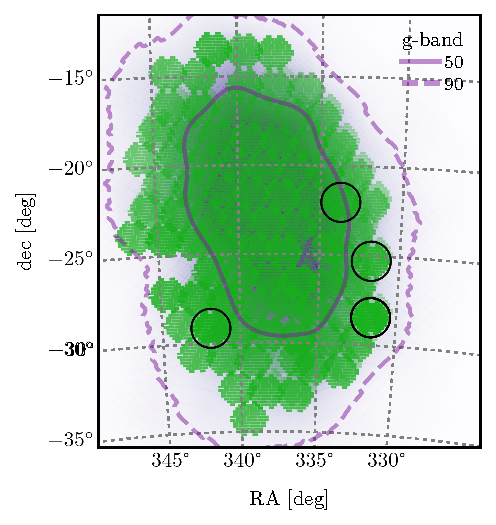
\includegraphics[width=0.49\textwidth]{figures/plot_followup_g.pdf}
    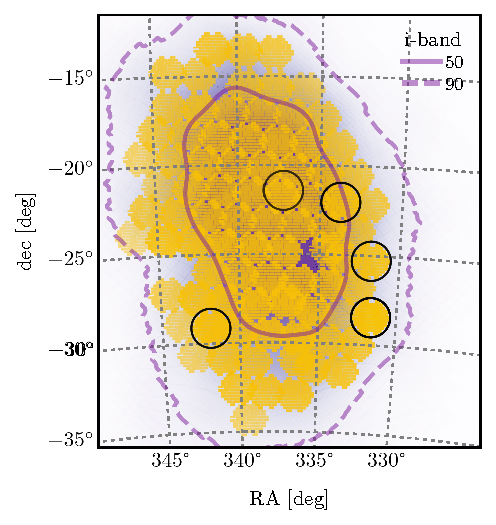
\includegraphics[width=0.49\textwidth]{figures/plot_followup_i.pdf}
    \caption{
        Our observation plan for follow up of \gweventid{}.
        The \gls{lvk} skymap for the event is plotted on the lower layers of the figure, and the 50\% (90\%) credible regions are outlined in the solid (dashed) line.
        The tiles circled in black are those in which the most interesting candidates were detected; extra observations of these tiles were conducted in addition to the full-tiling follow up plan.
    }
    \label{fig:plot_followup}
\end{figure}

Although we expect any \gls{em} counterpart to \gweventid{} to first become observable a few weeks after the \gls{lvk} detection, in light of uncertainties in the timescales of \gls{bbh} counterparts we decided to trigger our \gls{too} program for the night following the event (the evening of September 22, 2023).
Early observations following the merger also provide a baseline to identify \gls{agn} flares that rise after the \gls{gw} events, which is important considering that we do not typically have a rolling \gls{decam} survey to provide pre-merger observations in a generic \gls{gw} event localization.
Previous observations of the area are typically sparse and spread over a few years preceding the event.

On the first night we were only able to complete $\sim$1 hour of observations before inclement weather began, but we were able to observe our full plan in entirety the following night (September 23).
Further observations were conducted 11, 33, 41, and 70 days after the \gls{lvk} trigger (October 3, October 25, November 2, and December 1).
As we processed the data throughout the campaign, we took additional \gls{decam} observations of the most interesting candidates, adding 8 epochs altogether (the pointings for these supplementary observations are circled in Figure \ref{fig:plot_followup}).

We additionally used a variety of spectroscopic instruments to perform more detailed follow up of a short list of candidates; these candidates and data are described in \S\ref{subsec:cands}, where we discuss each candidate in particular.

\subsection{Transient discovery and vetting}

Our image differencing pipeline detected just over three million features in our campaign data, which we distilled into a tractable list of transients through a series of cuts.
Table \ref{tab:vetting} summarizes the vetting steps we applied, which are described in this section.

Data quality masks from the \gls{noirlab} \gls{decam} Community Pipeline were first applied to the list of difference image features to reduce the presence of instrumental noise.
Surviving features were then scored using a \gls{cnn} algorithm trained on archival \gls{decam} data products from our pipeline to perform real/bogus classification.
Possible real/bogus scores range from 0 to 1, with higher scores associated with more realistic objects; at this step we kept any detections with real/bogus scores greater than 0.7.
Roughly 7\% of the initial list of detections passed these steps to form our list of real astrophysical detections.

These detections were then cross-matched among themselves to identify features present in data from multiple epochs and discovered with multiple filters; the resulting list of transients consisted of 145,487 objects.
This list was subsequently cross-matched with the \gls{ls} and \gls{mpc} catalogs, and any transients respectively matched to a known variable star or minor planet were removed from our search.
A final automated vetting step was then applied to remove any transients which lacked observations separated by at least 30 minutes and those whose detections all had real/bogus scores below 0.9.
2,217 transients survived all of these cuts, from which human vetting identified 12 that were brightening by at least a few tenths of a mag on week-long timescales and/or were blue or getting more blue with time.
This list of 13 transients composed our short list that we performed supplementary \gls{decam} follow up of; the light curves for these transients are shown in Figure \ref{fig:light_curves_other_1} and \ref{fig:light_curves_other_2}.
These additional data narrowed our search to 4 candidates based on light curve morphology and colors.

\begin{table}[]
    \centering
    \begin{tabular}{c|c|c}
        Vetting filter & \# passed & \% passed \\
        \hline
        Initial photometry detections & 25,392,140 & 100 \\
        Data quality masking & 14,053,259 &  \\
        Real/bogus score $\ge$ 0.7 & 1,501,800 &  \\
        \hline 
        \multicolumn{3}{c}{\textit{Group detections into transient light curves}} \\
        \hline
        Initial transients & 233,313 & 100 \\
        Remove \gls{ls} variable stars & 140,230 & 60.1 \\
        Remove \gls{mpc} objects & 18,528 & 7.9 \\
        $\ge$1 real/bogus score $\ge$0.9 & 17,515 & 7.5 \\
        $\ge$2 detections with $\Delta t \ge 30$ & 3558 & 1.5 \\
        Human vetting & 13 & 0.0056
    \end{tabular}
    \caption{}
    \label{tab:vetting}
\end{table}

\section{Counterpart candidates to S230922g}

In this section we discuss especially interesting counterpart candidates to \gweventid{}.
These are either candidates for which we collected spectra for, or candidates with notable photometric light curves.
All of these candidates were classified with \gls{parsnip} \citep{booneParSNIPGenerativeModels2021}, with the resulting classification percentages shown in Table \ref{tab:parsnip}.

Spectroscopic observations served two purposes in our follow up campaign: to determine the nature of the host system, and to determine the nature of the transient itself.


\subsection{C202309242248405m134956}

Photometry, a spectrum, and sample stamps for this candidate are visible in Figure \ref{fig:light_curves_spectra_C202309242248405m134956}.

\begin{figure*}
    \centering
    \script{light_curves_spectra.py}
    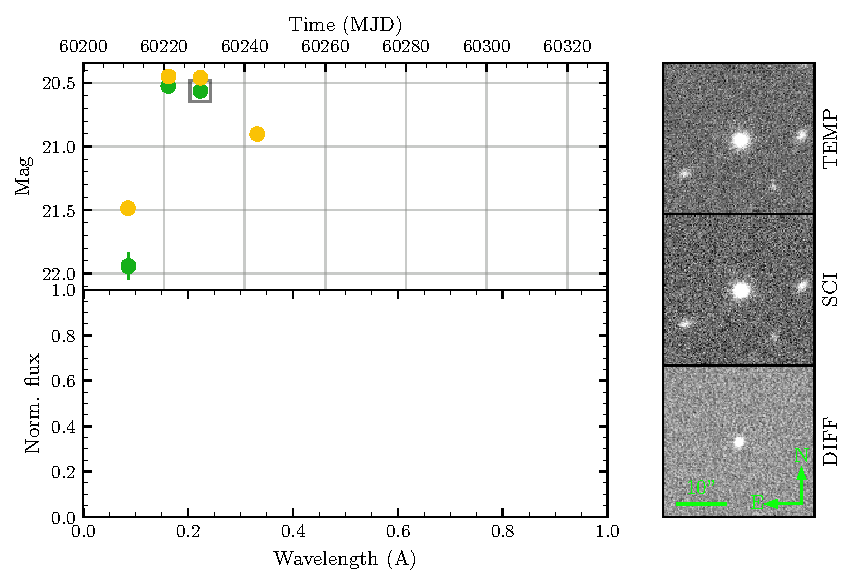
\includegraphics[width=0.95\textwidth]{figures/light_curves_spectra_7_C202309242248405m134956.pdf}
    \caption{
        Light curve, spectrum, and sample image stamps for the transient C202309242248405m134956.
        $g(i)$-band photometry is shown in green (yellow), and upper limits are indicated with hollow triangles.
        The stamps were taken from the data corresponding to the photometric point in the gray square.
        The colored vertical line in the light curve plot indicates the spectrum date.
        The spectrum for this event was taken with \todo{add telescope/instrument info.}
    }
    \label{fig:light_curves_spectra_C202309242248405m134956}
\end{figure*}

\subsection{A202310262246341m291842}

Photometry, a spectrum, and sample stamps for this candidate are visible in Figure \ref{fig:light_curves_spectra_A202310262246341m291842}.
This candidate was selected for spectroscopic follow up based on the significant brightening ($\sim$4 mag) exhibited at the onset of the transient.
The collected spectrum identifies the transient as a Type Ia \gls{sn} at a redshift of $\sim0.07$.


\begin{figure*}
    \centering
    \script{light_curves_spectra.py}
    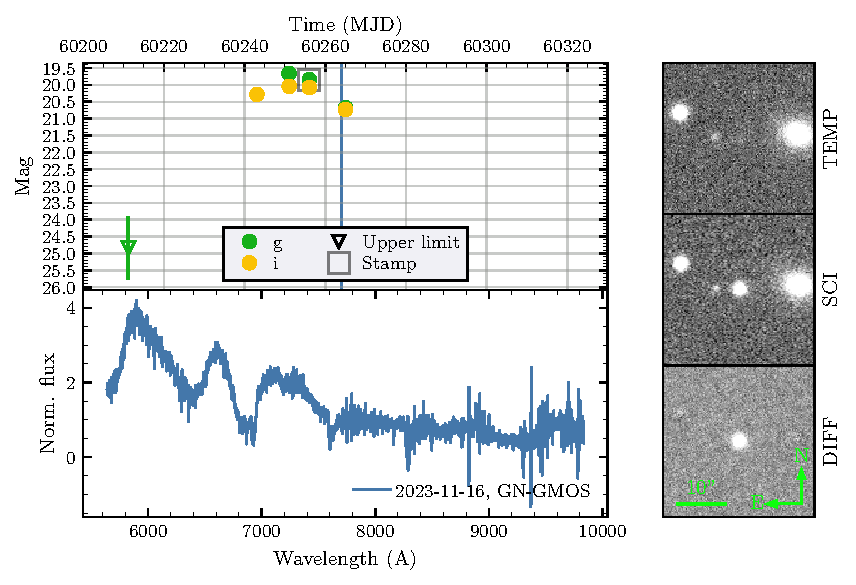
\includegraphics[width=0.95\textwidth]{figures/light_curves_spectra_7_A202310262246341m291842.pdf}
    \caption{
        As Figure \ref{fig:light_curves_spectra_C202309242248405m134956}, but for A202310262246341m291842.
        The spectrum for this event was taken with Gemini North GMOS.
    }
    \label{fig:light_curves_spectra_A202310262246341m291842}
\end{figure*}


\subsection{C202309242206400m275139}

Photometry, spectra, and sample stamps for this candidate are visible in Figure \ref{fig:light_curves_spectra_C202309242206400m275139}.
The transient was selected for spectroscopic follow up based on its persistent blue color and significant brightening.
The initial Keck spectrum revealed asymmetric broad line features for the H$\alpha$ and H$\beta$ regions, indicating an \gls{agn} host.
The redshift of the host was calculated to be 0.1838, placing the transient in the \todo{percentile} percentile for the \gweventid{} skymap.
An additional spectrum of the object was taken with Gemini North GMOS and reduced with DRAGONS \citep{labrieDRAGONSDataReduction2019} before the field set, with no noticeable attenuation of asymmetric features.



\begin{figure*}
    \centering
    \script{light_curves_spectra.py}
    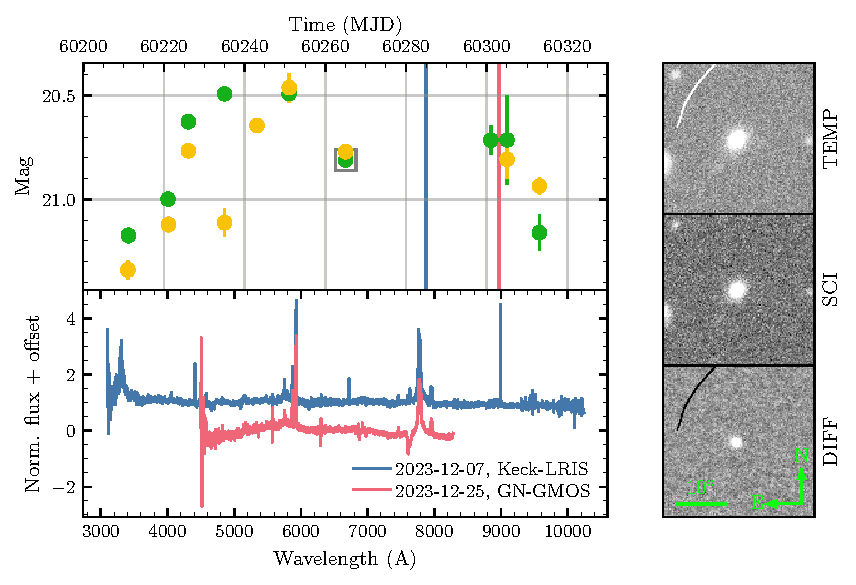
\includegraphics[width=0.95\textwidth]{figures/light_curves_spectra_15_C202309242206400m275139.pdf}
    \caption{
        As Figure \ref{fig:light_curves_spectra_C202309242248405m134956}, but for C202309242206400m275139.
        The first (second) spectrum for this event was taken with Keck LRIS (Gemini North GMOS).
    }
    \label{fig:light_curves_spectra_C202309242206400m275139}
\end{figure*}

\todo{Can we derive photometry from the spectrum for some additional points?}

\begin{figure*}
    \centering
    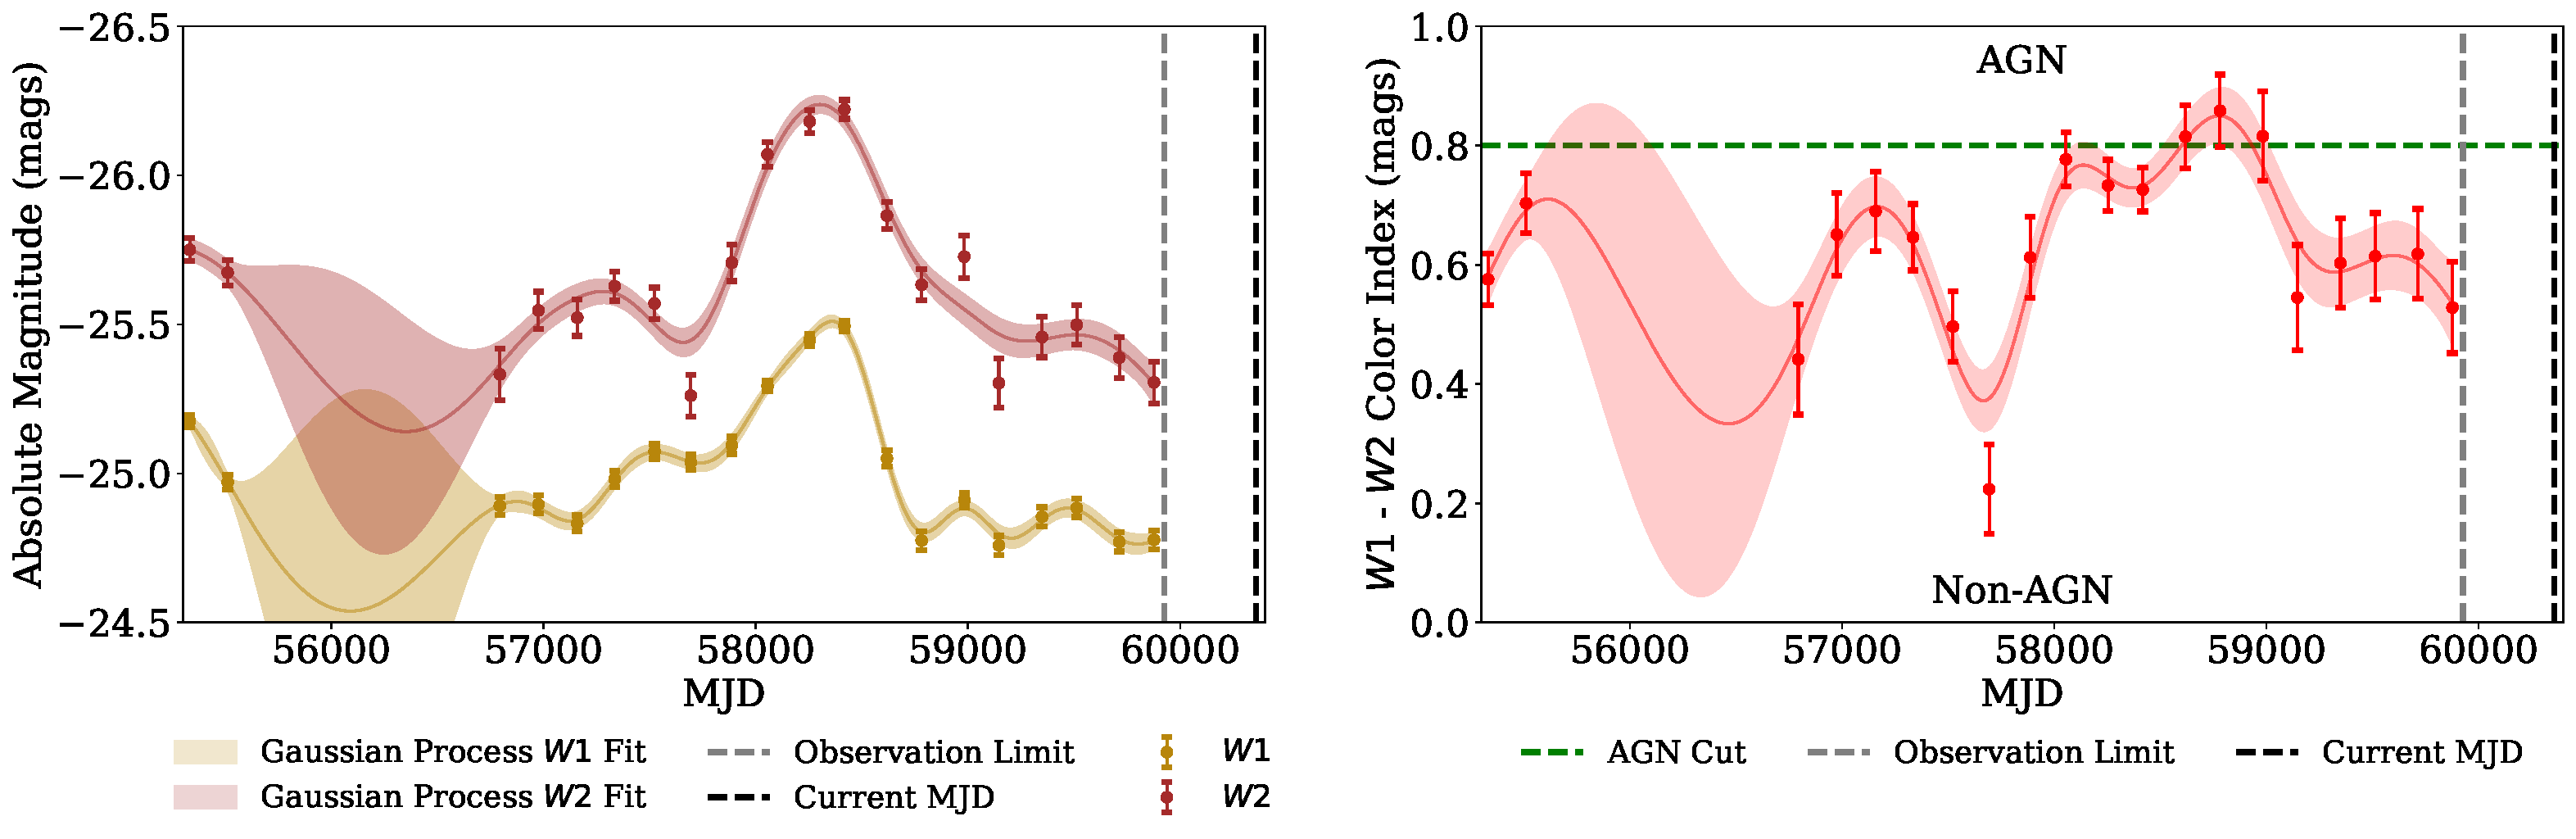
\includegraphics[width=0.95\textwidth]{figures/AT 2023aagj_MIR_Evolution.pdf}
    \caption{
        Archival WISE data for C202309242206400m275139.
    }
    \label{fig:WISE_C202309242206400m275139}
\end{figure*}

\subsection{C202310042207549m253435}

Photometry, a spectrum, and sample stamps for this candidate are visible in Figure \ref{fig:light_curves_spectra_C202310042207549m253435}.

\begin{figure*}
    \centering
    \script{light_curves_spectra.py}
    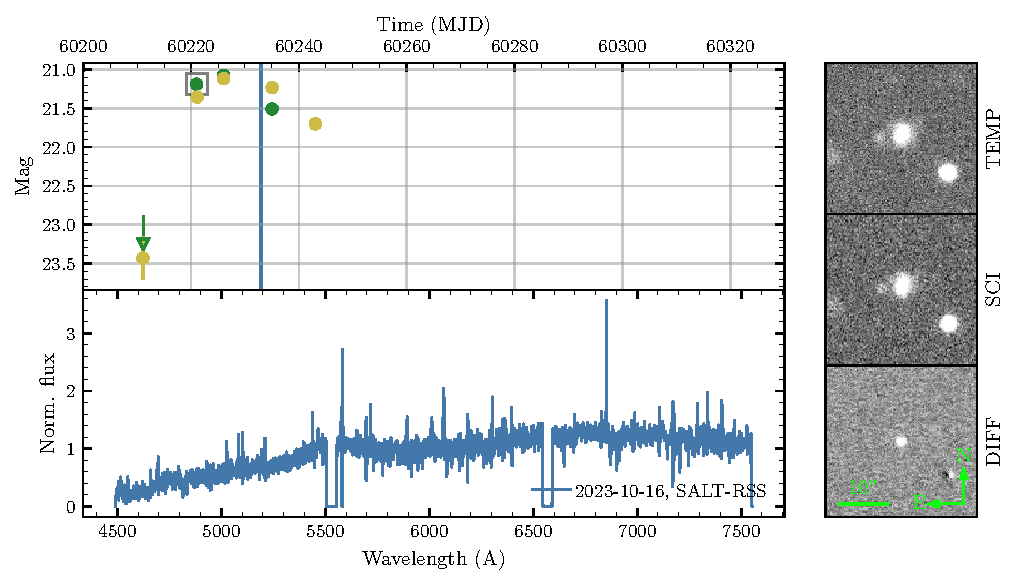
\includegraphics[width=0.95\textwidth]{figures/light_curves_spectra_7_C202310042207549m253435.pdf}
    \caption{
        As Figure \ref{fig:light_curves_spectra_C202309242248405m134956}, but for C202310042207549m253435.
        The spectrum for this event was taken with SALT RSS.
    }
    \label{fig:light_curves_spectra_C202310042207549m253435}
\end{figure*}

\begin{table*}[]
    \centering
    \begin{tabular}{c|c|c|c|c}
         & C202309242248405m134956 & A202310262246341m291842 & C202309242206400m275139 & C202310042207549m253435 \\
        \hline
        KN &  &  & 8e-4 &  \\
        SLSN-I &  &  & 8e-4 &  \\
        SNII &  &  & 0.029 &  \\
        SNIa &  &  & 0.019 &  \\
        SNIa-91bg &  &  & 9e-4 &  \\
        SNIax &  &  & 2e-3 &  \\
        SNIbc &  &  & 2e-3 &  \\
        TDE &  &  & \textbf{0.94} &  
    \end{tabular}
    \caption{
        \gls{parsnip} classifications of the \todo{four} transients described here; the highest classification category is indicated in bold.
    }
    \label{tab:parsnip}
\end{table*}

\begin{acknowledgements}

This material is based upon work supported by NSF Grant No. 2308193. This research used resources of the National Energy Research
Scientific Computing Center, a DOE Office of Science User Facility
supported by the Office of Science of the U.S. Department of Energy
under Contract No. DE-AC02-05CH11231 using NERSC award
HEP-ERCAP0029208 and HEP-ERCAP0022871. This work used resources on the Vera Cluster at the Pittsburgh Supercomputing Center. We thank T.J. Olesky and the PSC staff for help with setting up our software on the Vera Cluster.

This project used data obtained with the Dark Energy Camera (DECam), which was constructed by the Dark Energy Survey (DES) collaboration. Funding for the DES Projects has been provided by the US Department of Energy, the US National Science Foundation, the Ministry of Science and Education of Spain, the Science and Technology Facilities Council of the United Kingdom, the Higher Education Funding Council for England, the National Center for Supercomputing Applications at the University of Illinois at Urbana-Champaign, the Kavli Institute for Cosmological Physics at the University of Chicago, Center for Cosmology and Astro-Particle Physics at the Ohio State University, the Mitchell Institute for Fundamental Physics and Astronomy at Texas A\&M University, Financiadora de Estudos e Projetos, Fundação Carlos Chagas Filho de Amparo à Pesquisa do Estado do Rio de Janeiro, Conselho Nacional de Desenvolvimento Científico e Tecnológico and the Ministério da Ciência, Tecnologia e Inovação, the Deutsche Forschungsgemeinschaft and the Collaborating Institutions in the Dark Energy Survey.

The Collaborating Institutions are Argonne National Laboratory, the University of California at Santa Cruz, the University of Cambridge, Centro de Investigaciones En\`ergeticas, Medioambientales y Tecnol\`ogicas–Madrid, the University of Chicago, University College London, the DES-Brazil Consortium, the University of Edinburgh, the Eidgenössische Technische Hochschule (ETH) Zürich, Fermi National Accelerator Laboratory, the University of Illinois at Urbana-Champaign, the Institut de Ci\'encies de l’Espai (IEEC/CSIC), the Institut de F\'isica d’Altes Energies, Lawrence Berkeley National Laboratory, the Ludwig-Maximilians Universit\:at M\:unchen and the associated Excellence Cluster Universe, the University of Michigan, NSF’s \gls{noirlab}, the University of Nottingham, the Ohio State University, the OzDES Membership Consortium, the University of Pennsylvania, the University of Portsmouth, SLAC National Accelerator Laboratory, Stanford University, the University of Sussex, and Texas A\&M University.

Based on observations at Cerro Tololo Inter-American Observatory, NSF’s \gls{noirlab} (\gls{noirlab} Prop. ID 2022B-715089; PI: Palmese; and 2023B-851374 Prop. ID , PI: I. Andreoni \& A. Palmese), which is managed by the Association of Universities for Research in Astronomy (AURA) under a cooperative agreement with the National Science Foundation.
\textcolor{red}{Add Legacy Survey acknowledgements}
Slackbot: \url{https://github.com/scimma/slackbot} Ved Shah, Gautham Narayan, and the UIUCSN team

\end{acknowledgements}

\appendix

\begin{figure*}
    \centering
    \script{light_curves_other.py}
    \gridline{
        \fig{figures/light_curves_other_4_A202310042237432m160819.pdf}{0.49\textwidth}{}
        \fig{figures/light_curves_other_7_A202309242250535m165011.pdf}{0.49\textwidth}{}
    }
    \gridline{
        \fig{figures/light_curves_other_7_C202309242246522m280621.pdf}{0.49\textwidth}{}
        \fig{figures/light_curves_other_8_C202309242247183m132430.pdf}{0.49\textwidth}{}
    }
    \caption{Caption}
    \label{fig:light_curves_other_1}
\end{figure*}

\begin{figure*}
    \centering
    \script{light_curves_other.py}
    \gridline{
        \fig{figures/light_curves_other_8_T202310262246447m281410.pdf}{0.49\textwidth}{}
        \fig{figures/light_curves_other_10_C202309242214247m221046.pdf}{0.49\textwidth}{}
    }
    \gridline{
        \fig{figures/light_curves_other_13_C202309242244079m290053.pdf}{0.49\textwidth}{}
        \fig{figures/light_curves_other_19_C202309242204580m282926.pdf}{0.49\textwidth}{}
    }
    \caption{Caption}
    \label{fig:light_curves_other_2}
\end{figure*}

\section{Image processing}\label{sec:imgproc}

Our rapid image differencing pipeline can be divided into the following steps:
1) auxiliary data preparation, 2) science image preparation, 3) image subtraction, and 4) automatic transient vetting.

\subsection{Auxiliary data preparation}\label{subsec:auxdataprep}

After making an observing plan but before new data became available, we activate our pipeline to begin collection and organization of auxiliary data, which primarily take the form of template images and astronomical catalogs.

We use archival \gls{decam} images as templates for image differencing, selecting from the $>10^6$ exposures available in the \gls{noirlab} Astro Data Archive.\footnote{\url{https://astroarchive.noirlab.edu/}}
After updating a local \postgresql{} database of available image metadata, we compile a list of possible templates for a pointing out of those that
\begin{itemize}
    \item are within 0.05$^\circ$ of the pointing,
    \item predate the \gls{gw} trigger, and
    \item predate the observation night by $>$30 days.
\end{itemize}

We then assign each potential template a score equal to $t_{\rm exp} \cdot \teff$, where $t_{\rm exp}$ is exposure time and $\teff$ is the inverse ratio of $t_{\rm eff}$ to the historical exposure time required to produce an image of similar \gls{snr} ($\teff \to 1$ when the current conditions are near-optimal, and $\teff < 1$ when conditions are worse).
Practically, $\teff$ is computed as
\begin{equation}
    \teff
    \sim
    \frac{(10^{-0.4\texttt{cloudmag}})^2 * 10^{-0.4\texttt{skymag}}}{\texttt{FWHM}^2},
\end{equation}
where \texttt{cloudmag} is the cloud cover in magnitudes (\texttt{cloudmag} = 0 for clear skies, $>$ 0 for nonzero amounts of cloud cover), \texttt{skymag} is the sky brightness in magnitudes (\texttt{skymag} = 0 for dark skies, $>$ 0 for brighter skies), and \texttt{FWHM} is the FWHM of the guide stars used for the exposure, expressed in units of the historical median \citep{morgansonDarkEnergySurvey2018}.
Assigning each exposure a score of $t_{\rm exp} \cdot \teff$ provides information on both image depth and quality, facilitating a more holistic exposure assessment.
The image with the greatest score is chosen as the template for the respective pointing, with ties broken by largest $t_{\rm exp}$.
We use single archival images as our templates, as in practice the use of image stacks yields poor performance with our difference imaging software.

%%% Continue here 240209

Once suitable templates are selected for all pointings, our pipeline downloads the files for the respective exposures.
We label templates with the HEALPix indices for their coordinates, as a means of identifying each template as such for all exposures falling in the respective HEALPix tile.
This indexing, distinct from our custom tiling above during observing planning, ensures that our pipeline is flexible enough to process images that end up shifted due to pointing errors or manual pointing selection.

In this step our pipeline also collects catalog data for the planned observation area.
This includes \gls{ls} bricks containing morphologically-classified astrophysical sources, and an updated \gls{mpc} catalog.

\subsection{Science image preparation}\label{subsec:sciimgprep}

When the data for our follow-up exposures become available, we trigger the second step of our pipeline, which performs the final steps in organizing data for image processing.
Science images are labeled with HEALPix indices in the same manner as the templates (to ensure that exposures across epochs use the same template), and the \gls{ls} catalog data for each grouping is similarly linked.

\subsection{Image subtraction}\label{subsec:imgsub}

Image differencing begins resampling science images into alignment with templates using \texttt{SWarp} \citep{bertinTERAPIXPipeline2002}.
Image subtraction is completed with \gls{sfft} \citep{huImageSubtractionFourier2022}.
\gls{sfft} is a scalable image subtraction algorithm and GPU-enabled implementation of the same that produces difference images up to an order of magnitude faster than traditional tools while maintaining similar or exceptional product quality \citep{huImageSubtractionFourier2022}. 
Photometry on the science, template, and difference images is performed with \texttt{SExtractor} \citep{SExtractor}, and calibrated with the \gls{ls} source catalog.

The resulting list of candidates are distilled by analyzing their image stamps.
Any candidate whose stamps overlap with the \gls{cp} data quality masks for the respective exposures was rejected; this is checked for both the science (stamp size 5x5 pixels) and the template images (11x11 pixels).
We use a hybrid rotation-invariant CNN with ResNet18 \citep{2022FrASS...9.7100S} to perform real-bogus classification to vet spurious signals and image subtraction artifacts.
This model was trained on archival \gls{decam} data supplemented with transient simulations, and recovered 98\% of real/simulated transients with a bogus contamination of 7.2\%.
A single science exposure generally yields a few $\times 10^4$ candidates post-subtraction, approximately half of which pass data quality masking, of which $\sim15\%$ pass real/bogus classification, leaving a few thousand transient detections per exposure on average.

\subsection{Automatic transient vetting}\label{subsec:transvet}

Detected transients are then crossmatched with the \gls{ls} source and the \gls{mpc} catalogs.
Any objects not associated with objects in the \gls{mpc} catalog are categorized based on their proximity to \gls{ls} sources, distinguishing between star-type sources (identified with a \gls{ls} \texttt{TYPE} of ``PSF¨) and galaxy-type sources (all other \texttt{TYPE}s except \texttt{DUP}) \citep{sectionX.X,LS paper}.
Transients are classified into one of four categories in the following manner.


The pipeline is installed on both the \gls{nersc}-hosted Perlmutter and the \gls{psc}-hosted Vera supercomputing systems for redundancy and reliability.

\bibliography{DECam_first_O4_followup}

\end{document}
